\section{Perturbations, bootstrap coordinates, and use of the data}
\label{sec:physics-data-guide}

\subsection{Dimension-two operators and controlled deformations}

The absence of a relevant symmetry-invariant scalar has a precise but
limited meaning: it excludes an invariant scalar perturbation with
linearized RG eigenvalue $2-\Delta>0$. It does not settle the flow of
the dimension-two operators. For the diagonal theory all $36$ products
of vacuum currents are invariant under the full Verlinde category;
their nonabelian OPEs must still be taken into account.

There is nevertheless a concrete exactly marginal subfamily. Choose
the two Cartan currents and normalize them by
\[
 j^1=H_L/\sqrt2,\qquad j^2=H_R/\sqrt{78},\qquad
 j^a(z)j^b(0)\sim\frac{\delta^{ab}}{z^2}.
\]
Here $L,R$ label the two affine factors within one chirality, not the
two spacetime chiralities. The four local scalar fields
\begin{equation}\label{eq:physics-abelian-deformations}
 \mathcal O_{ab}(z,\bar z)=j^a(z)\overline{j^b}(\bar z),
 \qquad a,b\in\{1,2\},
\end{equation}
have the seed-point two-point functions
\[
 \langle\mathcal O_{ab}(z,\bar z)\mathcal O_{cd}(0)\rangle
 =\frac{\delta^{ac}\delta^{bd}}{|z|^4}.
\]
Thus the Zamolodchikov metric in this operator normalization is the
identity. The abelian current-current deformation criterion supplies
four simultaneous local exactly marginal directions
\cite[Section 2]{FR}. The associated current deformation space is locally
$O(2,2)/(O(2)\times O(2))$, before duality identifications. We do not
identify the complete conformal manifold or its global quotient.
Although these operators are categorical singlets at the rational
point, extending all topological lines and their junction data along
the deformation requires a separate argument. Exact marginality alone
does not prove that the entire deformed family retains the specified
Haagerup symmetry. In particular the count $36$ is not the dimension
of a claimed Haagerup-preserving conformal manifold.

The ordinary full $E_{8,1}$ theory has eight Cartan currents in each
chirality. Applying the same criterion gives the familiar $64$
toroidal deformation directions, locally
$O(8,8)/(O(8)\times O(8))$, at its enhanced-symmetry point. This
statement concerns the ordinary CFT; it does not identify which
deformations transport the specified Haagerup defect category.

\subsection{Coordinates for published exclusion plots}

For the ordinary scalar-gap bootstrap, allowing conserved currents,
the diagonal theory gives $(c,\Delta_{\rm scalar})=(8,2/3)$.
The holomorphic extension gives $(8,2)$, the familiar $E_{8,1}$ point
at the scalar-bound kink in Collier--Lin--Yin
\cite[Figure 8 and Section 3.3]{CLY}. Its ordinary bulk partition
function is the known $E_8$ one; the additional information here is
the specified Haagerup action and its relation to the explicit
subalgebra. The diagonal theory lies well below that scalar upper
bound. Chiral currents instead give the $E_8$ theory an all-primary
gap of one, so substituting that number in a scalar-gap plot would
compare different observables.

For the Haagerup bootstrap of Albert--Honda--Kaidi--Zheng, the physical
sector assignment in Section~\ref{sec:physics-H3} supplies
\begin{equation}\label{eq:physics-bootstrap-points}
 (c,\Delta_{\mathcal V_1}^{\rm scalar})=(8,2),\qquad
 (c,\Delta_{\mathcal V_{\pi_2}\cup\mathcal V_{\sigma_1}}^{\rm scalar})=(8,2).
\end{equation}
These are respectively the observables in Figures 2 and 3 of
\cite{AHKZ}. The multiplicity spaces $\mathcal V_\mu$ exclude the
finite-dimensional tube representation factors; the factor two in
the untwisted $\pi_2$ block must not be counted twice when constructing
the bootstrap vector. The $12$-sector vector for this comparison is
$\chi_\mu\overline{\chi_{E_8}}$, not the diagonal collection
$|\chi_\mu|^2$. The plots are numerical exclusions at the published
truncation, and our data do not rerun the associated semidefinite
program. In particular, the common value two is not by itself a
claim of saturation of either Haagerup bound.

Figure~\ref{fig:physics-Haagerup-bootstrap} places these two points on
the original published panels. Each point lies visibly below its
exclusion curve, in the shaded allowed region. We use this as a
consistency comparison, without extracting a numerical curve height
or claiming that the bounds single out this theory. The marker positions
are calibrated from the original axis ticks; the curves themselves
are reproduced without interpolation or refitting.
\begin{figure}[htbp]
 \centering
 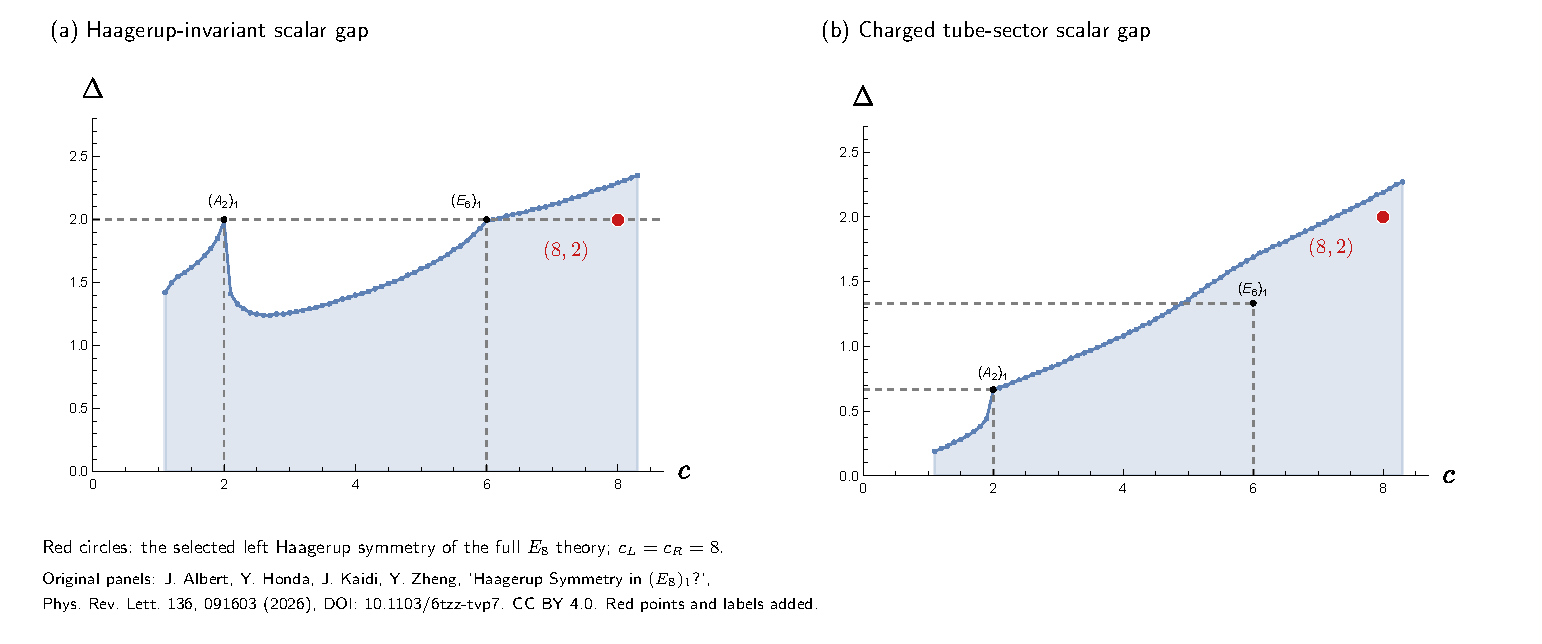
\includegraphics[width=\textwidth]{c8_physics_20260927/figures/haagerup_bootstrap_comparison.pdf}
 \caption{The $c_L=c_R=8$ Haagerup comparison points, shown in red.
 Original panels from J.~Albert, Y.~Honda, J.~Kaidi, and Y.~Zheng,
 \emph{Haagerup Symmetry in $(E_8)_1$?}, Phys.~Rev.~Lett.~136,
 091603 (2026), \href{https://doi.org/10.1103/6tzz-tvp7}{doi:10.1103/6tzz-tvp7},
 reproduced under CC~BY~4.0. Red markers and labels have been added.
 The left panel bounds $\mathcal V_1$; the right panel bounds
 $\mathcal V_{\pi_2}\cup\mathcal V_{\sigma_1}$.}
 \label{fig:physics-Haagerup-bootstrap}
\end{figure}

\subsection{Which observables are now supplied}

The release directory \artifact{c8_physics_20260927/} contains plain
TSV tables for inspection and JSON records retaining the algebraic
numbers, basis conventions, and exact derivations. There are four
distinct kinds of evidence.
\begin{enumerate}
 \item The character recurrence supplies complete spin-resolved state
 and Virasoro-primary spectra through $\Delta=24$, for both full
 theories. Thermodynamic intervals add a proved bound on the omitted
 tail, conditional on modular invariance and positivity.
 \item The actual lattice fields supply chiral vacuum-module
 three-point coefficients and the displayed four-point functions.
 Unit normalization and PCT are explicit. The current Ward completion
 of the weight-two tensor is checked against direct additional mode
 calculations.
 \item The positive modular data supply all Verlinde coefficients,
 diagonal-theory line eigenvalues, twisted partition functions and
 Cardy annuli. The selected extension and its free--forgetful
 adjunction supply the Haagerup-resolved $E_8$ sectors and boundaries.
 \item Universal CFT identities then give finite-size energies,
 momenta, entropy coefficients and the stress-tensor and current Ward
 observables. They do not determine the microscopic velocity $v$.
\end{enumerate}

The central unresolved interaction problem is the normalized bulk OPE
of the nonvacuum diagonal sectors, beginning with the nine scalar
components of dimension $2/3$. Neither their character coefficients
nor their fusion multiplicities determine their three-point constants.
An actual lattice intertwiner block, such as the example given above,
is useful input but must still be projected into channels and sewn
with consistent Hermitian pairings to obtain the full diagonal-CFT
four-point function. The corresponding numerical crossing tests,
general defect-junction correlators, and RG endpoints are not claimed
as outputs of this release. These are concrete follow-up calculations,
with the spectrum and normalization data here providing their starting
point.

Each exported number therefore has a mathematical location. Checking a
rational recurrence is separate from proving that its coefficients are
the characters of the constructed VOA; checking a lattice contraction
is separate from proving full-CFT sewing. This separation is intended
to make remaining gaps visible to both physicists and mathematicians.
